%!TEX root=000-main.tex

\chapter{Stateful Pipeline}

\todo{??}{
	
	Improve:
	\begin{itemize}
		\item Difference between stateless/stateful stage
		\item Stateful architecture pic
		\item Flow-states introduction
		\item Global-states introduction
	\end{itemize}
}

As defined by the OpenFlow specification, a packet entering an OpenFlow switch is processed through a set of linked flow tables that provide matching, forwarding, and packet modification. We indicate with the term \emph{stateless stage} the processing operated by a single legacy OpenFlow's flow table. Conversely, we define as \emph{stateful stage} (Figure~\ref{f:stateful-stage}) a logical stage comprising a state table and and a flow table, and implementing our abstraction.

\begin{figure}[h]
	\centering
	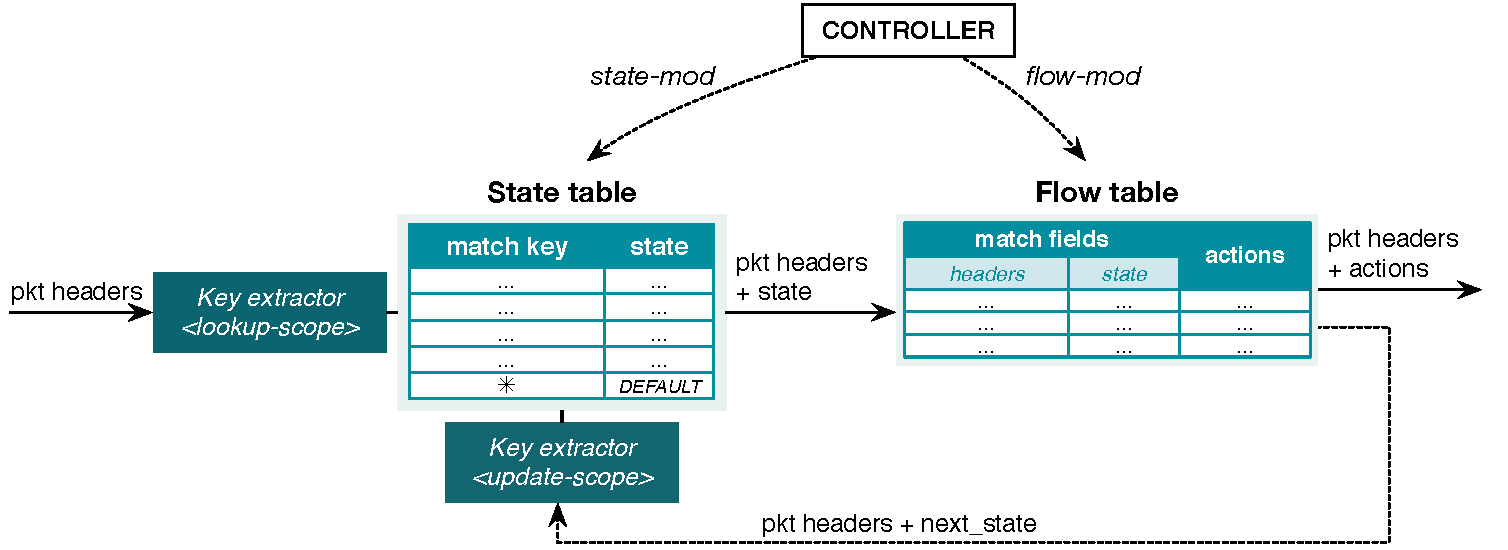
\includegraphics[width=\textwidth]{stateful-stage-arch}
	\caption{Architecture of an OpenState stateful stage}
	\label{f:stateful-stage}
\end{figure}

When a packet enters a stateful stage, it is first processed by a \emph{key extractor} which produces a string of bits representing the key to be used to match a row in the state table. The key is derived by concatenating the header fields defined in the \emph{lookup-scope}. The matched state label is appended to the packet headers as an additional header field. In case of a table-miss (the key is not matched) then a \emph{DEFAULT} state will be appended to the packet headers. If the header fields specified by the lookup-scope are not found (e.g. extracting the IP source address when the Ethernet type is not IP), a special state value \emph{NULL} is returned. By exiting the state table, packet headers along with the returned state label are matched in the flow table. A new \textbf{set-state} action to set the next state for the given flow is defined in the set of available OpenFlow actions.


A new switch capability has been defined in order to support all the OpenState functionalities, namely flow-states and global-states. By default all the flow tables in the switch are intended as stateless stages, the controller can then enable stateful processing for one or more stages by sending a special control message to the switch and by configuring the key extractors (lookup-scope and update-scope) associated with the state table. A new state modify message called \emph{state-mod} has been defined to allow the controller to configure the state entries and key extractors. Finally two new actions \textbf{set-state} and \textbf{set-flags} have been defined in order to respectively implement and configure the XFSM state transitions in the flow table and set the global states.